\chapter{Sensitivity Analysis} \label{ch:sa}

% - why deterministic
%     --> what is stochastic and why we can treat it as deterministic:
%         - stochasticity in the population synthesis
%         - stochasticity in the boarding priority (negligible)

% - borgonovo protocol
%         - outputs
%         - goal
%         - elements
%         - methods
%         - values
%         - visualization
        
% - visualizations & results & comments vari 


%%%%%%%%%%%%%%%%%%%%%%%%%%%%%%%%%%%%%%%%%%%%%%%%%%%%%%%%%%%%%%%%%%%%%%%%%%%%%%%%%%%%%%%

\section{Preliminaries} \label{sec:ch4_pre}

The first thing to understand in order to set up the sensitivity analysis of an agent-based model is whether the model under study is stochastic or deterministic. Let us recall the difference between the two frameworks: a model is \textit{deterministic}, if by fixing its input, the output remains unchanged when evaluating the model multiple times; alternatively, a model is \textit{stochastic} if it produces a random value any time it is run with the same fixed input. The nature of the model dictates the kind of output one is going to investigate and the course of the analysis to perform. In the case of a stochastic model, one would want to compute descriptive statistics of the conditional distribution of the output given the fixed values of the inputs, and this requires to evaluate a sufficient number of samples, in order to average out the random component in the output, making the analysis more computationally expensive. If the model is deterministic, instead, one simulation run per each value of the inputs is enough to be able to assess the uncertainty in the outputs. \\ So, before diving deep into the analysis, let us briefly recap the model under study in this research, which has been explained in detail in Chapter \ref{ch:model}, to understand its nature and plan the next steps of the analysis accordingly. The idea of the model is to reproduce the flow of passengers using Milan's transportation network, in order to evaluate the efficiency of the system.
\begin{figure}
    \centering
    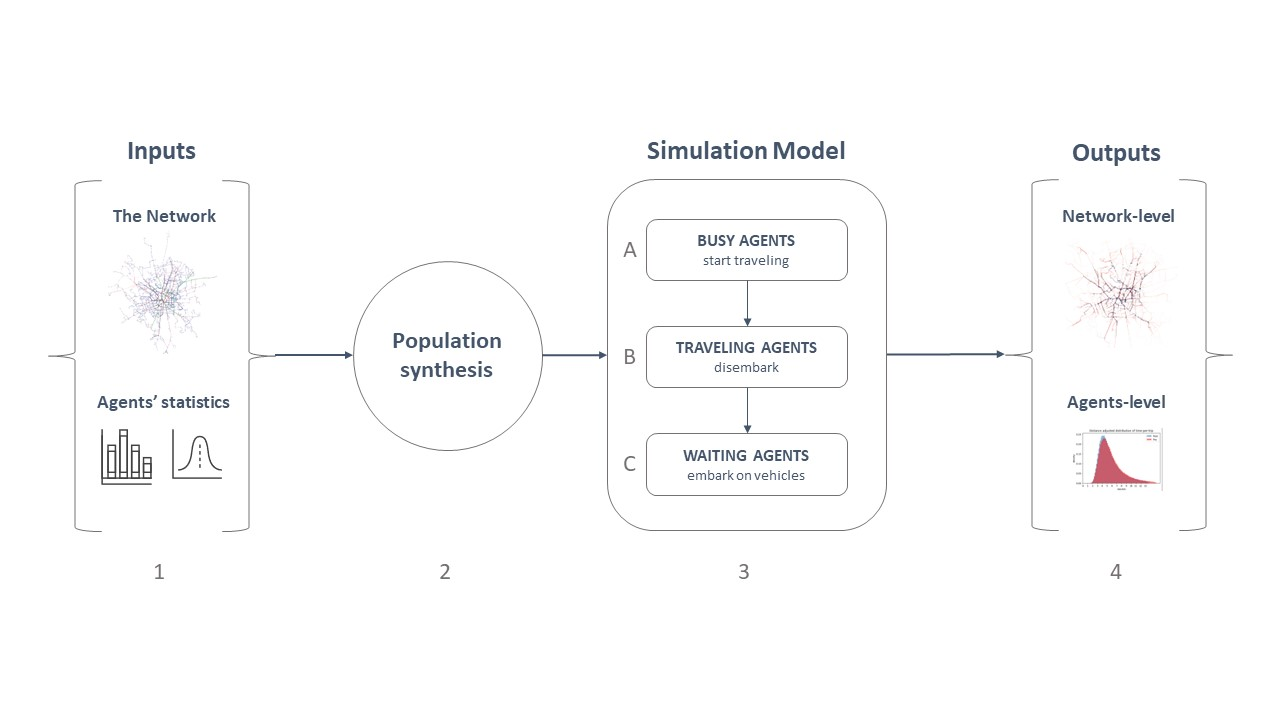
\includegraphics[width = \textwidth]{tex/pics/model_ppt2.jpg}
    \caption{Diagram representing the sequence of steps characterizing the agent-based model under study in this research.}
    \label{fig:model_schema}
\end{figure}
Figure \ref{fig:model_schema} portrays the main phases of the model. On the left side, there are the inputs that need to be fed to the simulator, which can be divided into those needed to construct the network, that will be the environment of the ABM, and those related to the distribution of agents' characteristics. Once one has collected all the inputs, the first step is to run the synthesis of the population. The goal of this phase is to obtain a fictitious population of agents which is as similar as possible to Milan's population, with respect to age, geographical residence and activities performed during an ordinary weekday. Next, the agents obtained are fed, together with the network, to the simulator: as soon as the simulation starts, they begin to move on the network to reach the location of the activities they have to perform. At the end of the simulation, the researcher is able to collect outputs related to the network (e.g. the most overloaded lines) or to the agents (e.g. traveling and waiting time), both at the individual and collective level. 
We can easily recognize two sources of stochasticity in the model's structure:
\begin{itemize}
	\item \textbf{The population synthesis} (2).
	\item \textbf{The boarding priority for waiting passengers} (B). 
\end{itemize}
I will now go through each of the two, in order to show that the impact of their stochastic nature on the model's results is negligible. In other words, for the purpose of the sensitivity analysis, from now on we will treat the model as if it were deterministic, that is, as if we obtain the same identical results from each model run, once the network, the population distributions and the number of agents has been fixed. This would allow us to perform one single run for each parameter setting and make the analysis less computationally expensive.

\paragraph{The population synthesis} 
As described in Section \ref{sec:3.3}, in order to construct the profile of each agent, features like age class, geographical residence and kind of activities performed are drawn from their respective distributions, which have been extrapolated from real demographic data about the residents of Milan. The population synthesis is, thus, a stochastic procedure, producing, at each run, a possibly different sample of agents. The problem with this stochasticity is that agents behavior in the simulations depend on their characteristics. In paricular, the probability of living in a specific zone of the city and that of performing a certain activity are conditional on the age class the agent belongs to, and how busy are agents is among the main drivers of traffic on the network. Moreover, agents' destinations depend on the activity they have to perform, which, again, depends on the age class. In an agent-based models, the results are determined by the collective behavior of agents. Hence, running the simulations with any specific set of individuals would lead to unique results and possibly to the emergence of a distinct phenomenon. For example, in our model, if the number of agents in a sample having the same destination is above average, then the results of the simulation would be biased, as they could show a particular overload on lines that lead to that specific destination. Since one wishes to eliminate, from the bias in the results, the component which depends on the population synthesis, a best practice would be to evaluate the model with multiple batches of agents and then agerage results across simulations. However, one can demonstrate that a large sample size ensures to achieve enough stability in the proportions of the agents' characteristics, across different samples resulting from the population synthesis procedure. That is, if the sample size is large enough, then the empirical distribution of agents will resemble the true distribution and one can decide to treat each sample as if they were equivalent, producing similar results. This kind of analysis can be included in the process of validating the population synthesis, as to assess its robustness. Indeed, in Section \ref{ssec:3.3.1}, I compared 100 samples of synthetic agents, of which I observed the distributions of multiple characteristics. Results show that, with a sample size of 20000, variability across samples is low. Hence, I decide to set default sample size to 20000 and disregard the stochasticity in the agents' profiles creation for the purposes of the sensitivity analysis.

\paragraph{Waiting agents' boarding priority}
As explained in \ref{sec:3.4}, at each timestep, agents are moved one at a time, and waiting agents are the last to move, as they are allowed to embark on the vehicle only after traveling agents disembark. While agents having to disembark are always allowed to do so (since there is no capacity associated to stops), those who have to get on a vehicle may be stopped by the constraint that such vehicle has already reached full capacity and forced to wait for the next available mean. Hence, for waiting agents the boarding order is important. Indeed, and allowing always the same agent to be the first to get on a vehicle would drastically reduce someone's waiting time and increase someone else's.
In principle, for the purpose of this analysis I am only interested in the collective behavior of agents, and I am not going to inspect agents' individual behavior, as to follow the main scope of the model, that is, evaluating the public transportation system as a whole. So, any boarding priority strategy would be equally valid. However, to be more realistic, I assign the priority with which waiting agents embark on their preferred vehicle at random. More formally, given $c$ the remaining capacity of the vehicle and $w$ the number of waiting agents, we treat each $j$ of the $w$ agents as if they had the same probability of being the $i$-th to embark, for $i = 1, ..., c$, that is, $P[O_j = i] = \frac{1}{c}$, where $O_j$ is the random variable representing the order of embarking for agent $j$. Intuitively, given a list of waiting agents, at each timestep the list is randomly shuffled, and the first in the list gets to be the first to move. This is not the only possible strategy. Indeed, one could think of moving agents according to some fixed index, but, as a consequence, the ones with lowest indices would always be the first to embark and to disembark, exhibiting unrealistically low waiting times, while the opposite would happen for the last agents evaluated. Alternatively, another possibility could be to follow a decreasing order in waiting time, letting the agents arrived earlier at each stop moving first. However, this strategy requires to make more computations at each timestep, while the adopted strategy seems a reasonable compromise which allows being realistic and avoids giving the first-mover advantage always to the same agents. The problem is that, being this a stochastic strategy, it may happen that running twice the simulation with the same sample of agents would lead to different individual results, meaning the same agent could be waiting more or less across different simulations with identical inputs. Since I am only going to evaluate aggregate results (e.g. mean traveling time, mean waiting time, ...) and neglect individual patterns, I can safely ignore the stochasticity in boarding priority and treat this step as deterministic. Being the boarding procedure the only source of stochasticity in the simulation model, we can conclude that there is no source of significant stochasticity and assume the model has deterministic nature.
%%%%%%%%%%%%%%%%%%%%%%%%%%%%%%%%%%%%%%%%%%%%%%%%%%%%%%%%%%%%%%%%%%%%%%%%%%%%%%%%%%%%%%%

\section{Sensitivity analysis steps} \label{sec:ch4_steps}

\paragraph{Output of interest}


\paragraph{Goal}


\paragraph{Elements}


\paragraph{Sensitivity method/design}


\paragraph{Assignment of values}


\paragraph{Results communication/visualization}



%%%%%%%%%%%%%%%%%%%%%%%%%%%%%%%%%%%%%%%%%%%%%%%%%%%%%%%%%%%%%%%%%%%%%%%%%%%%%%%%%%%%%%%

\section{Results and visualizations} \label{sec:ch4_res}